% Author: Izaak Neutelings (January 2021)
% http://pgfplots.net/tikz/examples/fourier-transform/
% https://tex.stackexchange.com/questions/127375/replicate-the-fourier-transform-time-frequency-domains-correspondence-illustrati
% https://www.dspguide.com/ch13/4.htm
\usepackage{amsmath}
\usepackage{tikz}
\usepackage{physics}
\usepackage[outline]{contour} % glow around text
\usepackage{xcolor}
\usetikzlibrary{intersections}
\usetikzlibrary{decorations.markings}
\usetikzlibrary{angles,quotes} % for pic
\usetikzlibrary{calc}
\usetikzlibrary{3d}
\contourlength{1.3pt}

\tikzset{>=latex} % for LaTeX arrow head


\definecolor{mygrey}{RGB}{167,192,224}

\definecolor{mybluegrey}{RGB}{120, 150, 184}
\definecolor{mycyangrey}{RGB}{137,190,198}


\definecolor{bluesquare}{RGB}{213,232,255}
\definecolor{cyansquare}{RGB}{193,234,241}

\definecolor{bluecontour}{RGB}{242,248,255}


\definecolor{myblue}{RGB}{0,0,166}
\definecolor{mycyan}{RGB}{167,192,224}
\definecolor{mygreen}{RGB}{167,192,224}
\definecolor{myorange}{RGB}{167,192,224}
\definecolor{myred}{RGB}{239,85,59}
\definecolor{mydarkred}{RGB}{167,192,224}
\definecolor{mypurple}{RGB}{167,192,224}
\colorlet{mydarkblue}{myblue!80!black}

% \colorlet{myred}{red!85!black}
% \colorlet{myorange}{orange!90!black!80}
% \colorlet{mydarkred}{myred!80!black}
\tikzstyle{xline}=[myblue,thick]
\def\tick#1#2{\draw[thick] (#1) ++ (#2:0.1) --++ (#2-180:0.2)}
\tikzstyle{myarr}=[myblue!50,-{Latex[length=3,width=2]}]
\def\N{90}




% SQUARE WAVE 
\def\xmin{-0.7*\T}   % min x axis
\def\xmax{6.0}       % max x axis
\def\ymin{-1.04}     % min y axis
\def\ymax{1.3}       % max y axis
\def\A{0.67*\ymax}   % amplitude
\def\T{(0.35*\xmax)} % period
\def\f#1{\A*4/pi/(#1)*sin(360/\T*#1*Mod(\t,\T))} 

% SYNTHESIS 3D
\newcommand{\tikzFourierTransform}[1]{
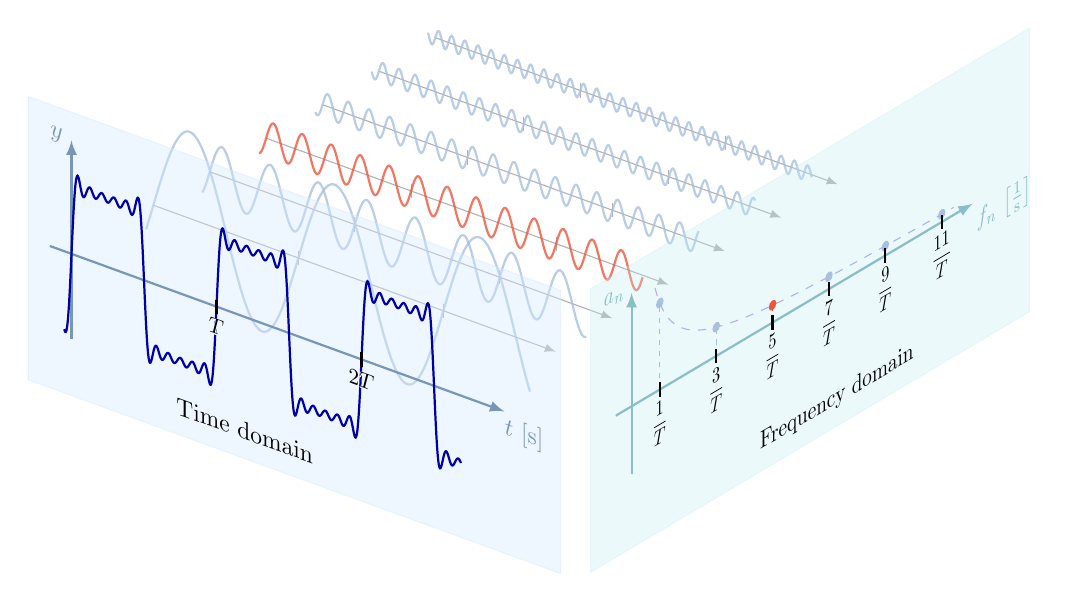
\begin{tikzpicture}[x=(-20:0.9), y=(90:0.9), z=(42:1.1)]
  \message{^^JSynthesis 3D}
  \def\xmax{6.5}        % max x axis
  \def\ymin{-1.2}       % min y axis
  \def\ymax{1.6}        % max y axis
  \def\zmax{5.8}        % max z axis
  \def\xf{1.17*\xmax}   % x position frequency axis
  \def\A{(0.60*\ymax)}  % amplitude
  \def\T{(0.335*\xmax)} % period
  \def\w{\zmax/11.2}    % spacing components
  
  % COMPONENTS
  \foreach \i/\col [evaluate={\z=\w*\i;}] in {
      11/mycyan,9/mypurple,7/myorange,5/myred,3/mygreen,1/mygrey}{
    \draw[black!30] ({\T},0.1,\z) --++ (0,-0.2,0);
    \draw[black!30] ({2*\T},0.1,\z) --++ (0,-0.2,0);
    \draw[->,black!30] (0,0,\z) --++ (0.93*\xmax,0,0);
    \draw[xline,\col,opacity=0.8,thick,
          samples=\i*\N,smooth,variable=\t,domain=-0.05*\T:0.87*\xmax]
      plot(\t,{\f{\i}},\z);
  }
  
  % TIME DOMAIN
  \begin{scope}[shift={(0,0,-0.17*\zmax)}]
    \draw[bluesquare,fill=bluesquare,opacity=0.4,canvas is xy plane at z=0]
      (-0.1*\xmax,-1.25*\ymax) rectangle (1.13*\xmax,1.25*\ymax);
    \draw[->,mybluegrey,thick] (-0.05*\xmax,0,0) -- (\xmax,0,0)
      node[below right=-3,canvas is xy plane at z=0] {$t$ [s]};
    \draw[->,mybluegrey,thick] (0,\ymin,0) -- (0,\ymax,0)
      node[left,canvas is xy plane at z=0] {$y$};
    \draw[xline,myblue,thick,
          samples=9*\N,smooth,variable=\t,domain=-0.05*\T:0.9*\xmax]
      plot(\t,{\f{1}+\f{3}+\f{5}+\f{7}+\f{9}+\f{11}},0); %node[above] {$f$};
    \tick{{\T},0,0}{90}
      node[below=-1,scale=0.9,canvas is xy plane at z=0] {\contour{bluecontour}{$T$}};
    \tick{{2*\T},0,0}{90}
      node[below=-1,scale=0.9,canvas is xy plane at z=0] {\contour{bluecontour}{$2T$}};
    \node[scale=1,canvas is xy plane at z=0] at (0.4*\xmax,-\ymax,0) {Time domain};
  \end{scope}
  
  % FREQUENCY DOMAIN
  \begin{scope}[shift={(\xf,0,0)}]
    \draw[cyansquare,fill=cyansquare,opacity=0.3,canvas is zy plane at x=0]
      (-0.13*\zmax,-1.25*\ymax) rectangle (1.26*\zmax,1.25*\ymax);
    %\draw[->,thick] (0,0,0) -- (0,0,\zmax) node[above left=-1] {$z$};
    %\draw[->,thick] (\xmax,0,0) --++ (0,0,\zmax);
    \draw[->,mycyangrey,thick] (0,0.8*\ymin,0) -- (0,\ymax,0)
      node[above=2,left=0,canvas is zy plane at x=0] {$a_n$};
      %node[pos=0.84,left=2,fill=white,inner sep=0] {$b_n$};
    \draw[->,mycyangrey,thick] (0,0,-0.05*\zmax) --++ (0,0,1.13*\zmax)
      node[below right=-1,canvas is zy plane at x=0] {$f_n$ $\left[\frac{1}{\mathrm{s}}\right]$};
    \node[scale=1,canvas is zy plane at x=0] at (0,-\ymax,0.65*\zmax) {Frequency domain};
    \draw[myblue!30,dashed,samples=3*\N,smooth,variable=\t,domain=0.074*\zmax:1.02*\zmax]
      plot(0,{\A*4/pi/\t*\w},\t); %node[right=2,above=0,scale=0.7] {$\dfrac{4A}{\pi n}$};
    \foreach \i/\col [evaluate={\z=\w*\i;}] in {
        11/mycyan,9/mypurple,7/myorange,5/myred,3/mygreen,1/mygrey}{
      \draw[\col,dash pattern=on 2 off 2]
        (0,0,\z) --++ (0,{\A*4/pi/\i},0);
      \fill[\col,canvas is zy plane at x=0]
        %(\xf,{\A*4/pi/\i},\z) circle(0.08);
        (\z,{\A*4/pi/\i}) circle(0.07);
      \tick{0,0,\z}{90}
        node[below=-1,scale=0.85,canvas is zy plane at x=0]
        {$\dfrac{\i}{T}$}; %f_\i=\ifnum\i=1 \else \i \fi T
    }
    % \foreach \i [evaluate={\z=\w*\i;}] in {2,4,...,10}{
    %   \fill[myblue!60!black,canvas is zy plane at x=0] (\z,0) circle(0.07);
    % }
  \end{scope}
  
\end{tikzpicture}

}